\chapter{High Symmetry Paths for Sulfosalt Band Structure Calculations}\label{paths}

The high-symmetry points of the Brillouin zones of the crystal structures being studied here are shown in figure \ref{brill} and given in units of reciprocal lattice vectors in table \ref{symm_points}, which were taken from the Bilbao Crystollographic Server \cite{Bilbao, Bilbao2}.
The high symmetry lines for each of the crystal structures are shown in equations \ref{31} and \ref{36} where equation \ref{31} shows the high symmetry lines for the crystal structure Pmn2$_1$, which is that of enargite ({\enargite}) and bournonite ({\bournonite}), and equation \ref{36} shows the high symmetry lines for crystal structure Cmc2$_1$, which is that of stephanite ({\stephanite}).

\begin{equation}\label{31}
R \longrightarrow S \longrightarrow X\longrightarrow\Gamma \longrightarrow Y \longrightarrow T \longrightarrow Z \longrightarrow U
\end{equation}

\begin{equation}\label{36}
R \longrightarrow S \longrightarrow \Gamma \longrightarrow Y \longrightarrow T \longrightarrow Z \longrightarrow \Gamma
\end{equation}

Calculations of the electronic band structure in this study are performed using the FHI-aims DFT code \cite{aims}, which was described in the section above.
In practise, this is implemented in the FHI-aims code by requesting the band structure along the high symmetry lines shown in equations \ref{31} and \ref{36} to be outputted from a starting point, such as the $\Gamma$ point, to an end point such as Y with a certain number of points in between, which determines how smooth the plot will appear.

\begin{figure}[h!]
  \centering
    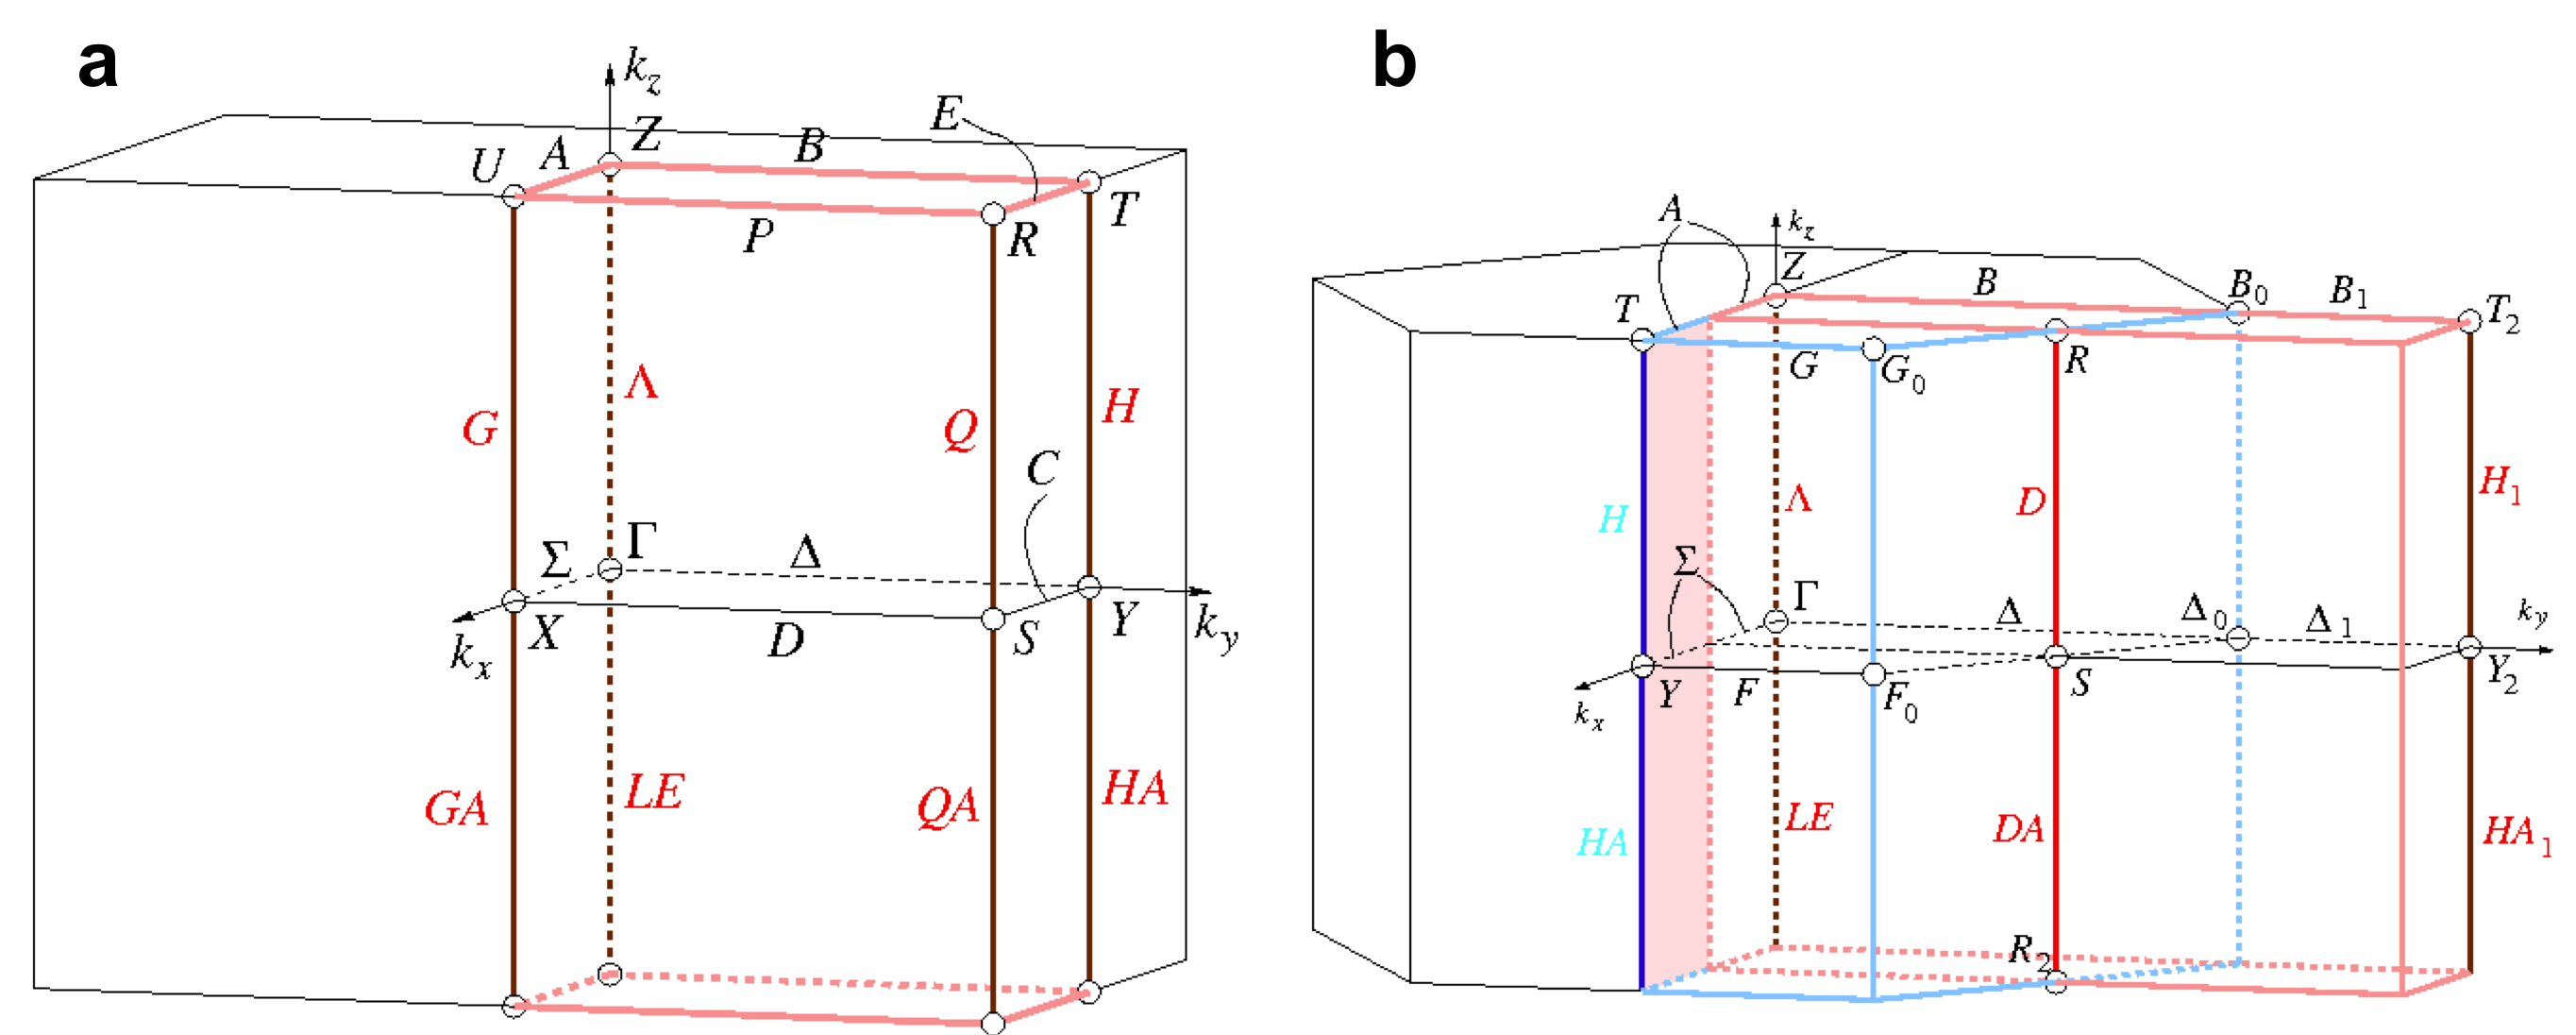
\includegraphics[width=1.0\textwidth]{figures/brill.png}
    \caption{The reciprocal lattice shown with the first Brillouin zone for the space groups Pmn2$_1$ (a) and Cmc2$_1$ (b), where the former is the space group of enargite ({\enargite}) and bournonite ({\bournonite}) and the latter is the space group of stephanite ({\stephanite}). Figures taken from the Bilbao Crystallographic Server \cite{Bilbao, Bilbao2}.}
  \label{brill}
\end{figure}

\begin{table}[]
\centering
\caption{High symmetry points for the Pmn2$_1$ and Cmc2$_1$ given in units of reciprocal lattice vectors (\textbf{k} = $x_1\mathbf{b_1} + x_2\mathbf{b_2} + x_3\mathbf{b_3}$), taken from the Bilbao Crystallographic Server \cite{Bilbao, Bilbao2}.}
\label{symm_points}
\begin{tabular}{llll|llll}
\toprule[1.2pt]
\multicolumn{4}{c}{Pmn2$_1$}     & \multicolumn{4}{c}{Cmc2$_1$}     \\
         & $x_1$ & $x_2$ & $x_3$ &          & $x_1$ & $x_2$ & $x_3$\\  \midrule[1pt]
R        & 0.5   & 0.5   & 0.5   & R        & 0     & 0.5   & 0.5   \\
S        & 0.5   & 0.5   & 0     & S        & 0     & 0.5   & 0     \\
X        & 0.5   & 0     & 0     & $\Gamma$ & 0     & 0     & 0     \\
$\Gamma$ & 0     & 0     & 0     & Y        & 0.5   & 0.5   & 0     \\
Y        & 0     & 0.5   & 0     & T        & 0.5   & 0.5   & 0.5   \\
T        & 0     & 0.5   & 0.5   & Z        & 0     & 0     &       \\
Z        & 0     & 0     & 0.5   & $\Gamma$   & 0     & 0     & 0     \\
U        & 0.5   & 0     & 0.5   &          &       &       &      
\\ \bottomrule[1.2pt]
\end{tabular}
\end{table}